\documentclass{article}
\usepackage[a4paper, total={18cm, 26cm}]{geometry}
\usepackage{fixme}
\usepackage{algorithm}
\usepackage{algpseudocode}
\usepackage{amsmath}
\usepackage{url}
\usepackage{fixme}
\usepackage[utf8]{inputenc}
\usepackage{graphicx}
\usepackage{subcaption}

% Keywords command
\providecommand{\keywords}[1]
{
  \small	
  \textbf{\textit{Keywords---}} #1
}

\title{{RILS}: Regression via Iterated Local Search for Symbolic Regression GECCO Competition -- 2023}

\author{Aleksandar Kartelj$^{1}$, Marko Djukanovi\'{c}$^{2}$  \\
        \small $^{1}$University of Belgrade, aleksandar.kartelj@gmail.com \\
        \small $^{2}$University of Banja Luka, marko.djukanovic@pmf.unibl.org \\
}
\date{}

\begin{document}
\maketitle

\begin{abstract} % abstract
We describe a program pipeline for solving symbolic regression problems. The main element of this pipeline is the sequential search algorithm based on Iterated Local Search. The main components of the algorithm are a carefully designed local search procedure and the incremental solution construction, i.e., the search that iteratively increases the limit of the expression size. The sequential algorithm (base regressor) is later used in a parallel environment in the form of an ensemble of regressors.
After additional post-processing of the results obtained by the ensemble, we report the following results: \texttt{dataset\_1} ($R^2$=0.8385, size=55), \texttt{dataset\_2} ($R^2$=0.9547, size=17) and \texttt{dataset\_3} ($R^2$=0.9789, size=43).
\end{abstract}

\keywords{symbolic regression, iterated local search, incremental construction, GECCO 2023, competition}

\section{Short introduction}

Recently, we proposed a method called RILS-ROLS for dealing with symbolic regression (SR)~\cite{kartelj2023_rils_rols}. It was able to outperform the other (14) literature approaches in terms of (symbolic) solution rate on the two well-known ground truth benchmark sets from the literature~\cite{la2021contemporary}, in the presence of different noise levels.

RILS is a modified and in some sense simplified version of RILS-ROLS, better suited for dealing with the datasets of the SR competition at GECCO '23.
The changes from RILS-ROLS and the new features can be summarized as follows:

\begin{itemize} 
\item RILS does not use ordinary least squares (OLS) to adjust coefficients within linear combinations -- this is done using an internal dynamic coefficient tuning procedure. 
\item One-perturbations are examined randomly, not systematically as in RILS-ROLS. 
\item RILS uses a local search with randomized first-improvement strategy, unlike RILS-ROLS, which uses best-improvement local search strategy. 
\item The fitness function is different, i.e., it considers only $R^2$ with a fixed upper bound on the expression complexity, and this upper bound is monotonically increased during the search. 
\item RILS does not consider solutions dominated by a previous solution in terms of solution complexity and $R^2$, so the set of Pareto-optimal solutions is preserved during the search. This was not the case for RILS-ROLS. 
\item There are two post-processing steps, while RILS-ROLS did not use post-processing.
\end{itemize}

We will first describe the RILS method, which will later be used as the main component of the overall RILS-based pipeline.

\section{RILS method}\label{sec:rils}

Our method relies on the following operations $+$, $-$, $\cdot$, $/$, and the elementary mathematical functions $\sqrt{x}$, $x^2 $, $\sin$, $\cos$, $\log$ and $\exp$. In addition, the following set of constants enters the search space explicitly: $-1$, $0$, $0.5$, $1$, $2$, $e$, $\pi$, and $10$. The RILS scheme is shown in Algorithm 1.   

\begin{algorithm}
	\footnotesize
\begin{algorithmic}[1] 
\Statex	  \textbf{Input}: input training dataset $D_{tr}$  
\Statex \textbf{Parameters}: $init$ ("0"), $target_{size}$ (20), $fitCalls_{max}$ (100000), $seconds_{max}$ (10000), $seed$ (0)
    \Statex \textbf{Output}: best symbolic formula solution $best$
    \State $best \gets init$ 
    \State $best_{fit} \gets$ \texttt{Fitness}($best, D_{tr}$)
        \State $pareto_{set} \gets \{ best_{fit} \}$
    \While{\emph{stopping criteria is not met}}
    \State $best_{perturbations} \gets $ \texttt{All1Perturbations}($best$) \label{line:sPert}
        \State $pert \gets $ \texttt{RandomPick}($best_{perturbations}$) \label{line:pickPert}
       \State $pert \gets $ \texttt{LocalSearch}($pert$, $D_{tr}$) \label{line:ls}
    \State $pert_{fit} \gets$ \texttt{Fitness}($pert$, $D_{tr}$)
    \If{$pert_{fit} < best_{fit}$ and not \texttt{Dominated}($pert_{fit}, pareto_{set}$)} \label{line:avoid1}
    \State $best, best_{fit} \gets pert, pert_{fit}$ // new best solution
        \State \texttt{AddAndUpdate}($best_{fit}, pareto_{set}$)
    \EndIf \label{line:avoid2}
    \EndWhile
    \State \Return $best$
\end{algorithmic}
\caption{RILS method.}
\end{algorithm}

The \textsc{RILS} method receives the training dataset $D_{tr}$ as input. It also has two important control parameters: the initial solution $init$ and the size of the target expression $target_{size}$. There are some other standard parameters such as the maximum number of fitness function evaluations ($fitCalls_{max}$), the maximum execution time ($seconds_{max}$), and the pseudo-random number generator seed ($seed$). The default initial solution is the expression "0". Non-zero solutions are used within an ensemble of regressors; this is described in Section~\ref{sec:rils_ensemble}. The $target_{size}$ represents, as the name implies, the preferred size of the expression (effectively an upper bound, since expressions of smaller size are not explicitly penalized). The target size is enforced in two ways: 1) by penalizing larger expressions through the fitness function, and 2) by avoiding transformations (within the local search) that increase the size of the solution expression.

The main loop iterates until none of the termination criteria are met: ($i$) the maximum runtime has been reached; ($ii$) the maximum number of fitness calculations has been performed. One of the first steps in the main loop is to generate perturbations near the current best solution $best$ (line~\ref{line:sPert}).
As the name of this procedure (\texttt{All1Perturbations}) implies, the perturbation step is local, i.e. the proximity between the best solution $best$ and any perturbation is 1 (therefore we call it 1-perturbation). The perturbation generation step is described in~\cite{kartelj2023_rils_rols}. In the next step, a random perturbation $pert$ is selected from the perturbation set, after which a local search (line~\ref{line:ls}) is performed on $pert$. The local search generates neighboring candidate solutions near $pert$. The set of candidates is similar to \cite{kartelj2023_rils_rols}. The main difference is that the set of candidates is reduced to those with size at most $target_{size}$. Also, unlike in \cite{kartelj2023_rils_rols}, where the best-improvement strategy was used, here we use the randomized first-improvement strategy. This means that the set of candidates must be randomly shuffled before the probing. The adjustment of the coefficients is also done as part of the local search. This means that a substantial portion of the candidates for the local search is obtained by multiplying each coefficient within the model by the following set of multipliers $\pm\{0.01, 0.1, 0.5, 0.8, 0.99, 1, 1.2, 2, 10, 100\}$.

Finally, the fitness function value of $pert$ is compared with the fitness function value of $best$ and with the set of all Pareto fitness values. (Although the comparison with the Pareto fitness set is sufficient since $best_{fit}$ must lie in it, it is more efficient to check whether the $pert$ fitness is at all suitable to be compared with the $pareto_{set}$ by first comparing $pert_{fit}$ and $best_{fit}$) The fitness function is given in Equation~(\ref{eq:fitness}).
 
\begin{equation}
	\label{eq:fitness}
	fitness(s) = (2-R^2(s)) \cdot \max(target_{size}, size(s))
\end{equation}

Since RILS tries to minimize fitness, a lower value for $2-R^2(s)$ implies a higher value for $R^2$. The second part of the fitness function is related to expression size: all solutions less than $target_{size}$ are considered as solutions of size $target_{size}$. It turns out that this fitness function behaves \emph{well} when solutions are built incrementally, which is the case in the RILS ensemble, i.e., the $target_{size}$ is increased in subsequent iterations. The reason for this is likely that the search algorithm can focus on the $R^2$ objective and no tradeoffs within this specified subspace of solutions (with size at most $target_{size}$) are required.

Another point worth mentioning is that, like RILS-ROLS, RILS uses the mechanism of expression caching, which on average speeds up the search process by a factor of two, i.e., the cache hit rate is about 50\%. For more details on expression caching, see \cite{kartelj2023_rils_rols}.

\section{RILS-ensemble method}\label{sec:rils_ensemble}

RILS can be run concurrently (preferably in parallel) using method called RILS-ensemble. The ensemble is based on multiple RILS regressors with different settings of the $seed$ parameter. The method is outlined in Algorithm 2.

\begin{algorithm}
\footnotesize
\begin{algorithmic}[1]
    \Statex	  \textbf{Input}: input training dataset $D_{tr}$  
    \Statex \textbf{Parameters}: $init$ ("0"), $initTarget_{size}$ (20), $epochs$ (100), $epochFitCalls_{max}$ (100000), $epochSeconds_{max}$ (10000), $parallelism$ (10)
    \Statex \textbf{Output}: best symbolic formula solution $best$
    \State $best \gets init$ 
    \State $best_{fit} \gets$ \texttt{Fitness}($best, D_{tr}$)
    \State $target_{size} \gets initTarget_{size}$
    \For{\texttt{$epoch \gets 1 ... epochs$}}
        \State $regressors \gets []$
        \For{\texttt{$seed \gets 1 ... parallelism$}}
            \State $regressors.append$(RILS($best, target_{size},epochFitCalls_{max},epochSeconds_{max},seed$)
        \EndFor
        \State $epochBest, epochBest_{fit} \gets $ \texttt{ParallelCall}($regressors$)\label{line:parCall} 
        \If{$epochBest_{fit} < best_{fit}$}
            \State $best, best_{fit} \gets epochBest, epochBest_{fit}$
        \Else
            \State $target_{size} \gets target_{size} + 1$
        \EndIf
    \EndFor
    \State \Return $best$
\end{algorithmic}
\caption{RILS-ensemble method.}
\end{algorithm}

The set of RILS ensemble control parameters is similar to the RILS parameters. In addition, there are the following parameters: $epochs$ -- the number of ensemble calls, $parallelism$ -- the number of regressors within the ensemble. Also, the $target_{size}$ parameter is now called $initTarget_{size}$, since this parameter is no longer fixed as in RILS, but increases with epochs.
The main loop iterates over epochs. In each epoch, the ensemble of regressors is built. The parameter that is different for each regressor is $seed$. The parameter $init$ is set to the current $best$ solution, while the parameter $target_{size}$ is set to the active target size of the ensemble, which increases over epochs. Therefore, the parameters $init$ and $target_{size}$ vary over epochs, but are the same for each regressor in the fixed epoch. The remaining RILS parameters $fitCalls_{max}$ and $seconds_{max}$ are constant across epochs, and their values are set to $epochFitCalls_{max}$ and $epochSeconds_{max}$, respectively. Once the ensemble is built, it is called with a parallel call (line~\ref{line:parCall}). When execution is complete, the best symbolic model of all regressors is selected and compared to the current $best$. If there is an improvement, $best$ and $best_{fit}$ are updated accordingly. Otherwise, the $target_{size}$ is increased.

\section{Overall RILS pipeline}\label{sec:rils-pipeline}

The entire RILS pipeline is adapted to competition datasets and therefore cannot be considered general. Nevertheless, we believe that the building blocks such as RILS and RILS-ensemble are general enough to be applied to a variety of datasets. The pipeline steps for each of the three datasets considered are as follows:
\begin{enumerate}
    \item RILS-ensemble is run with the following parameters: $init="0"$, $epochFitsCalls_{max}=100000$, $epochSeconds_{max}=10000$, and $parallelism=10$. For \texttt{dataset\_1} and \texttt{dataset\_3}, initial experiments showed that the expected expression sizes are larger than for \texttt{dataset\_1}, making \texttt{dataset\_2} much easier to solve. Therefore, we used $initTarget_{size}=10$ for \texttt{dataset\_2}, while we used $initTarget_{size}=20$ for the other two datasets. Also, the search for \texttt{dataset\_2} converged much faster, so we evaluated it for only 100 epochs, while the convergence was much slower for the other two datasets, so we set $epochs=180$. The search was done on 75\% of available data, i.e., 1500 data points. 
    \item RILS-ensemble stores the best solution for each epoch. Since $target_{size}$ increases with epochs, the stored solutions \emph{kind of} form a Pareto set with non-decreasing $R^2$ values and mostly increasing solution expression sizes. So the second step is to choose the best trade-off solution from all these solutions. There are several ways to do this. The best known approach is to choose an \emph{knee} (or sometimes called elbow) point. There are also more complex approaches in the literature. We have chosen an approach similar to the \emph{knee} approach, i.e., we go through the solutions with increasing $R^2$ and stop when the $R^2$ undergoes the last relevant increase. The relevant $R^2$ increase is set to 0.005 (0.5\%) in our approach. 
    \item The next step is an automated approximate simplification: a) we remove expression parts whose absence does not cause significant $R^2$ degradation; more precisely, we remove the expression part if the $R^2$ decrease divided by the size decrease is less than 0.001 (0.1\%). 
    \item The last step is the semi-automatic simplification. We use the method \texttt{nsimplify} from the package \texttt{Sympy}~\cite{sympy}) to approximately unify similar coefficients (if this change does not significantly worsen $R^2$). This step also includes ad-hoc simplifications that are clearly visible to the naked eye but difficult for a program to detect. This simplification was only useful in the case of \texttt{dataset\_3} and will be discussed in more detail in this section.
\end{enumerate}

The program is implemented in Python 3.11.3, but should also work with other relatively recent versions of Python 3. All experiments on our method are performed in multi-core mode on a PC with Intel i9-9900KF CPU @3.6GHz, 64GB RAM, running Windows 10 Pro OS. All codes, datasets and instructions for reproducing the results are available at: \\ \url{https://github.com/ufabc-bcc/srbench-competition-2023-track-1-sarma/}.

\section{Experimental results}

The final results are shown in Table~\ref{tab:results}. They are obtained by evaluating the models using SR competition scripts, therefore, they consider all 2000 data points.

\begin{table}[ht]
 \renewcommand*{\arraystretch}{1.4}
    \footnotesize
    \caption{Results of \textsc{RILS Ensemble} on the three given datasets (using all training data).}
    \centering
    \begin{tabular}{l |lrr} \hline
    Datasets & Solution (rounded to two decimals) & $R^2$   &  size  \\ \hline \hline
      \texttt{dataset\_1}  &
      \parbox{10cm}{
      \begin{equation}
      \nonumber
    \begin{aligned}
      \approx & (-1.37\cdot \sin(3.18\cdot x_0 + 9.88) + e^{-0.33\cdot x_0}\cdot \sin(2.43\cdot x_0)) 
      \\ &\cdot (-1.84\cdot x_1 - (3.26 - 0.79\cdot x_1)\cdot \sin(1.18\cdot x6) + 7.55)
      \\ & \cdot (-0.02\cdot e^{x_6} + 0.47\cdot \cos(2.90\cdot x_6 - 1) + 0.06)\cdot \cos(2.90\cdot x_1 - 1) 
      \end{aligned}
      \end{equation}
      }
      & 0.8385 & 55 \\ \hline
      \texttt{dataset\_2}  & 
      \parbox{10cm}{
      \begin{equation}
      \nonumber
      \approx x_0\cdot x_5^3\cdot(0.31\cdot x_4 + 2.4)\cdot \sin(x_6)^{1/4}/x_3
    \end{equation}
      } & 0.9547 & 17\\ \hline
      \texttt{dataset\_3}  & 
      \parbox{10cm}{
       \begin{equation}
      \nonumber
        \begin{aligned}
      & (\sin(10\cdot \ln(x_0))+ \sin(10\cdot \ln(x_1)) + \sin(10\cdot \ln(x_4)) + \sin(10\cdot \ln(x_5)) \\
      &+ \sin(10\cdot \ln(x_6)) +  \sin(10\cdot \ln(x_7)) + \sin(10\cdot \ln(x_{10})) + \sin(10\cdot \ln(x_{11})))/8
      \end{aligned}
      \end{equation}}
       & 0.9789 & 43\\ \hline
    \end{tabular}
    \label{tab:results}
\end{table}

Figure~\ref{fig:fig_tradeoff} shows the solution sets obtained after step 1 of the RILS pipeline (on training data, i.e., 1500 data points). We will now focus only on \texttt{dataset\_3}, since the other two data sets are fully automated and they give the presented results without step 4 of the RILS pipeline.

In Step 2, the best trade-off solution for \texttt{dataset\_3} is selected that achieves (size, $R^2$)=(119, 0.9766). This solution is reduced in step 3 to a solution with (size, $R^2$)=(91, 0.9724), which has the following structure:

\begin{equation}
\nonumber
\begin{aligned}
    &0.12707266214999\cdot \sin(10\cdot \ln(x_1)) + 0.121515728046397 \cdot \sin(10 \cdot \ln(x_{10})) + 0.11599065741255\cdot \sin(10\cdot \ln(x_{11})) \\
    &+ 0.124768331044259\cdot \sin(10\cdot \ln(x_5)) + 0.128296185170387\cdot \sin(10\cdot \ln(x_6)) - 0.117968516690417\cdot \sin(\ln(x_7^{-10})) \\
    &- 0.128553858459013\cdot \cos(10.37539750401 \cdot \ln(108.821/x_0) + \sin(\ln(x_0^{0.5}))) \\
    &- 0.125960699057812\cdot \cos(16.84644380626584/x_4^{0.5} - 2 \cdot \ln(x_4 + 0.418907513197396)^{2} \\
    &+ 0.576\cdot \cos(12\cdot \sin(1/(x_4 + 1)) + 0.72) - 0.1275897046702296)
\end{aligned}
\end{equation}

From then on, we used the \texttt{nsimplify} method in interactive mode to further simplify the expression. First, it became clear that all factors were multiplied by a number of 0.125 (1/8), which is very close to the average coefficient in all linear terms. Then, all $cos$ were converted to $sin$, while the subexpression $-0.125 \cdot \sin(\ln(x_7^{-10}))$ was converted to $0.125 \cdot \sin(10\ln(x_7))$. Finally, using the notion of self-similarity in linear terms, we were able to convert the complicated expressions with variables $x_0$ and $x_4$ inside the former $cos$ terms to $10 \cdot \ln(x_0)$ and $10 \cdot ln(x_4)$, respectively, leading to the final form of the solution:

\begin{equation}
\nonumber
\begin{aligned}
\frac{\sin(10 \ln(x_0))+ \sin(10 \ln(x_1)) + \sin(10 \ln(x_4)) + \sin(10 \ln(x_5)) +\sin(10 \ln(x_6)) +  \sin(10 \ln(x_7)) + \sin(10 \ln(x_{10})) + \sin(10 \ln(x_{11}))}{8}.
\end{aligned}
\end{equation}

This simplification also led to an improvement in terms of $R^2$, so that the final model is (size, $R^2$)=(43, 0.9789).

\begin{figure}[ht]
\begin{subfigure}{.5\textwidth}
  \centering
  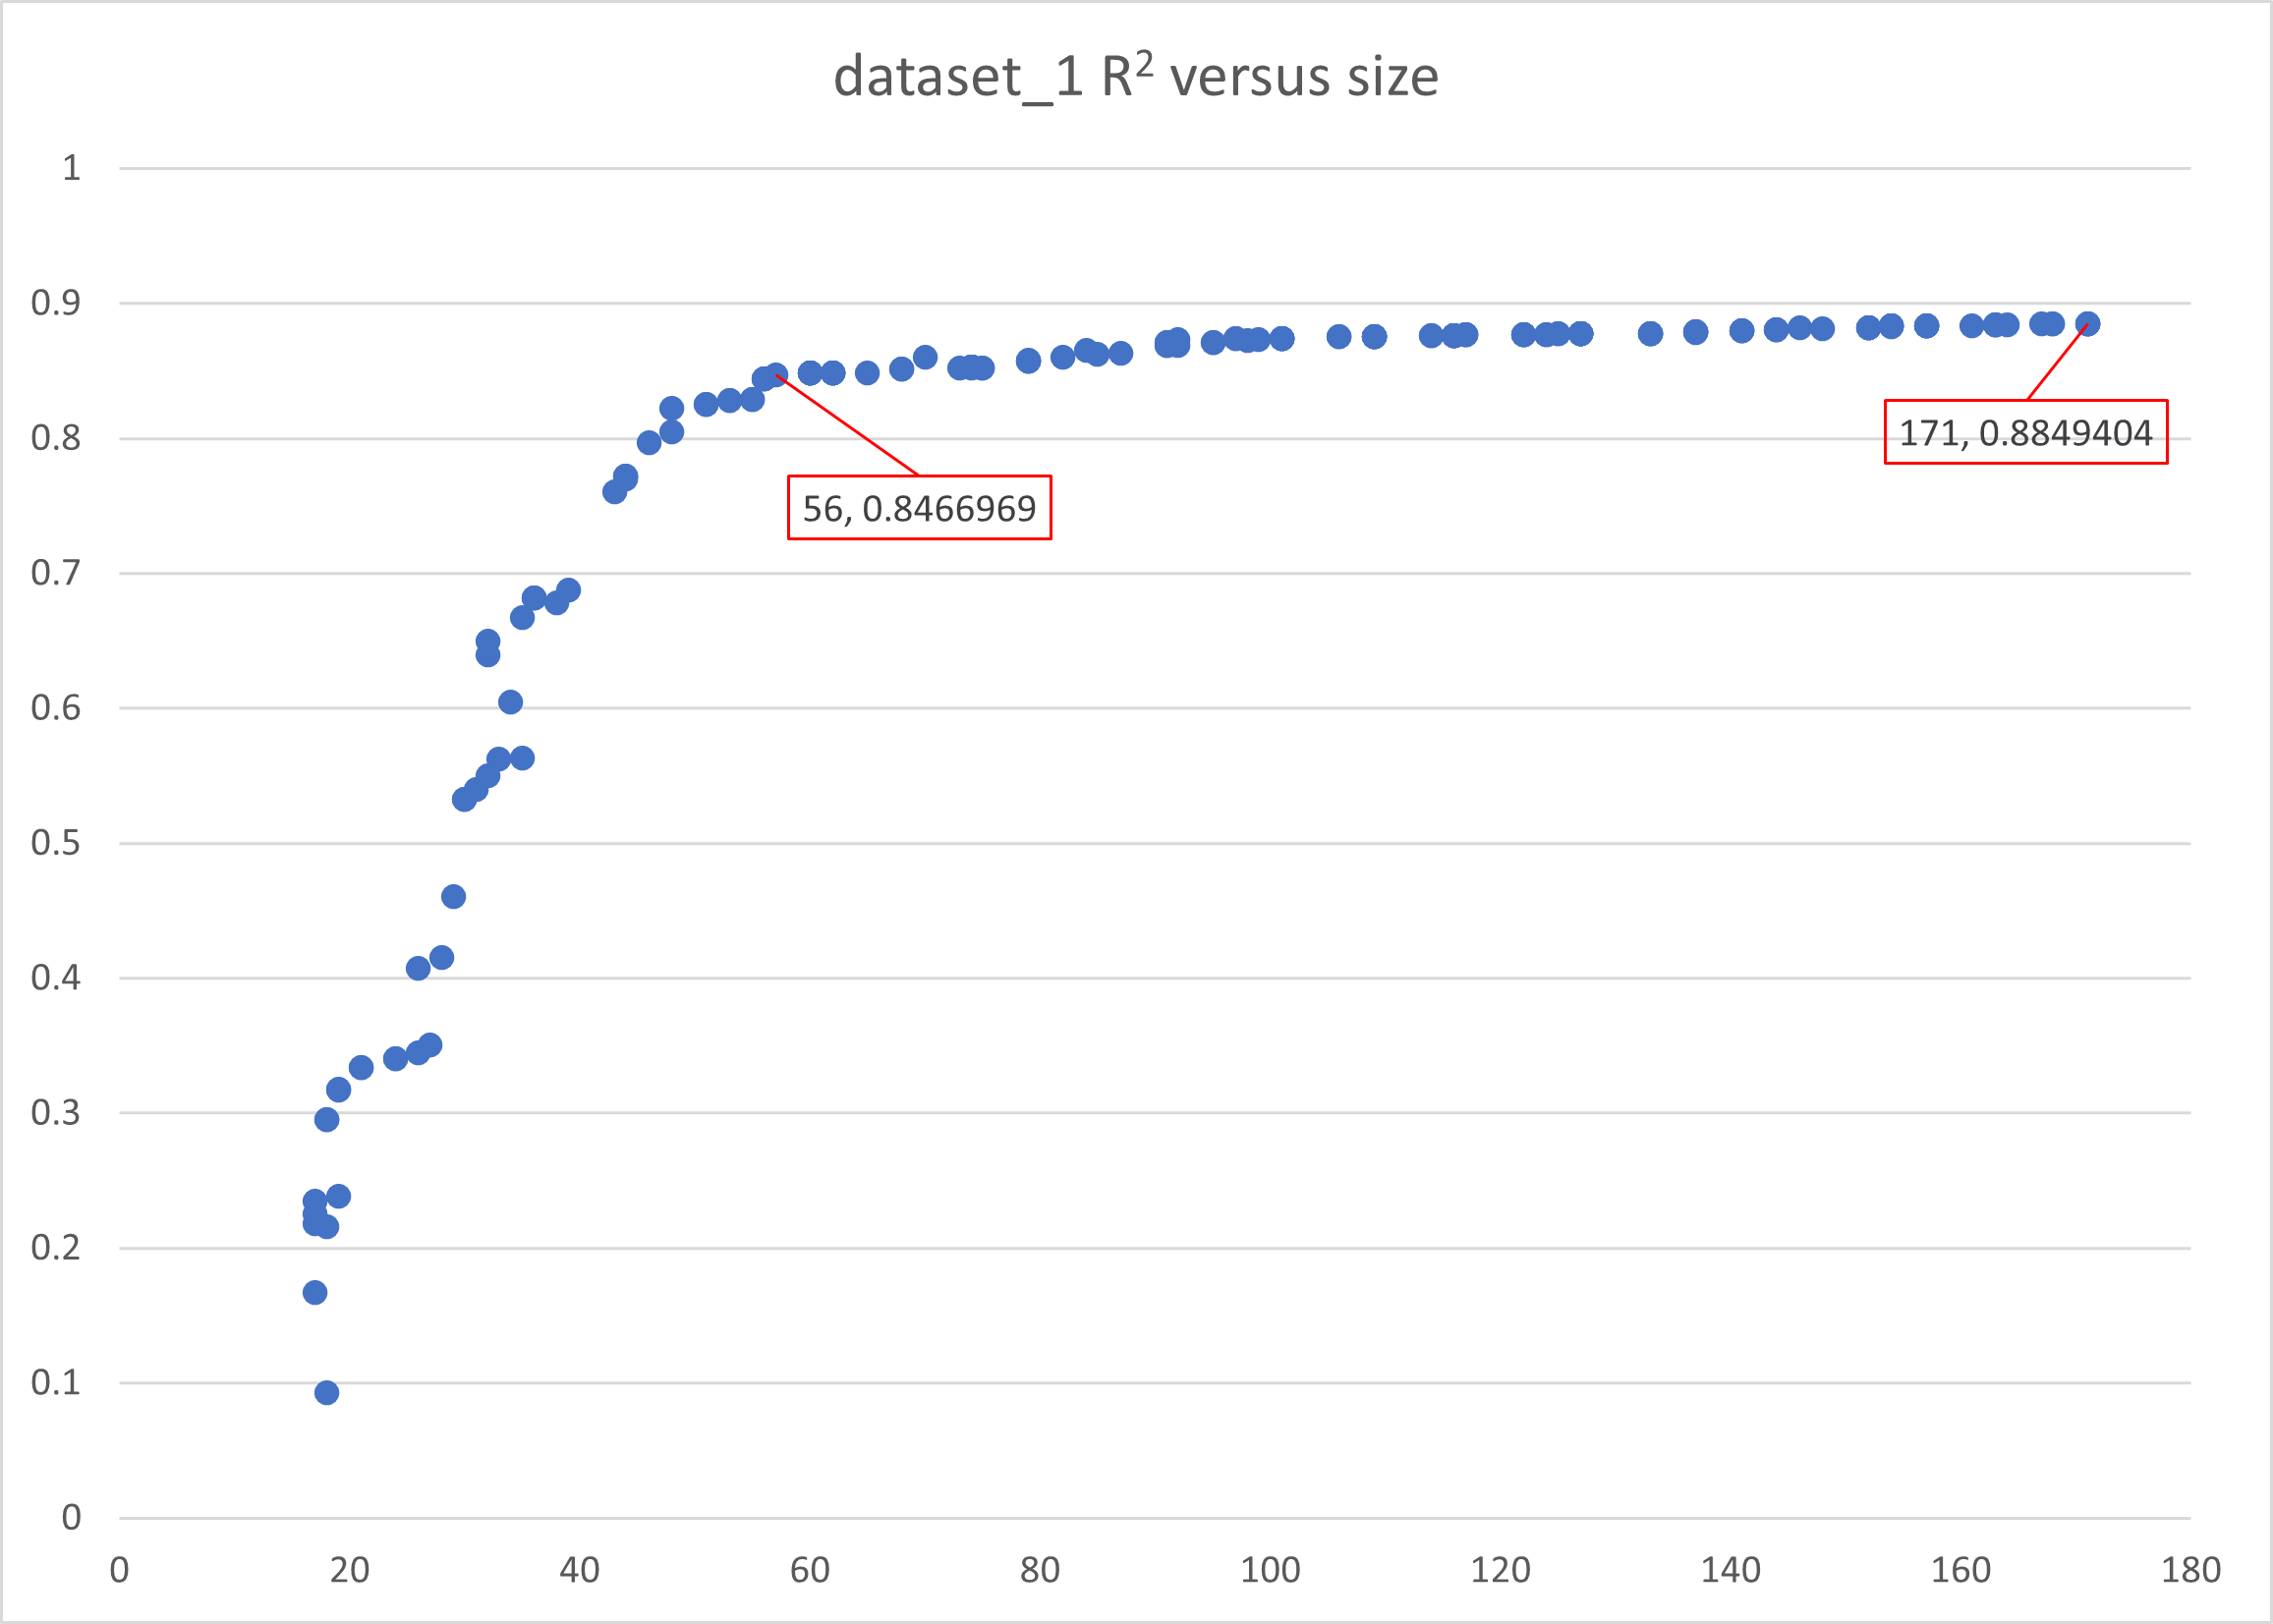
\includegraphics[width=0.95\linewidth]{solutions1.png}
  \label{fig:sfig1}
\end{subfigure}%
\begin{subfigure}{.5\textwidth}
  \centering
  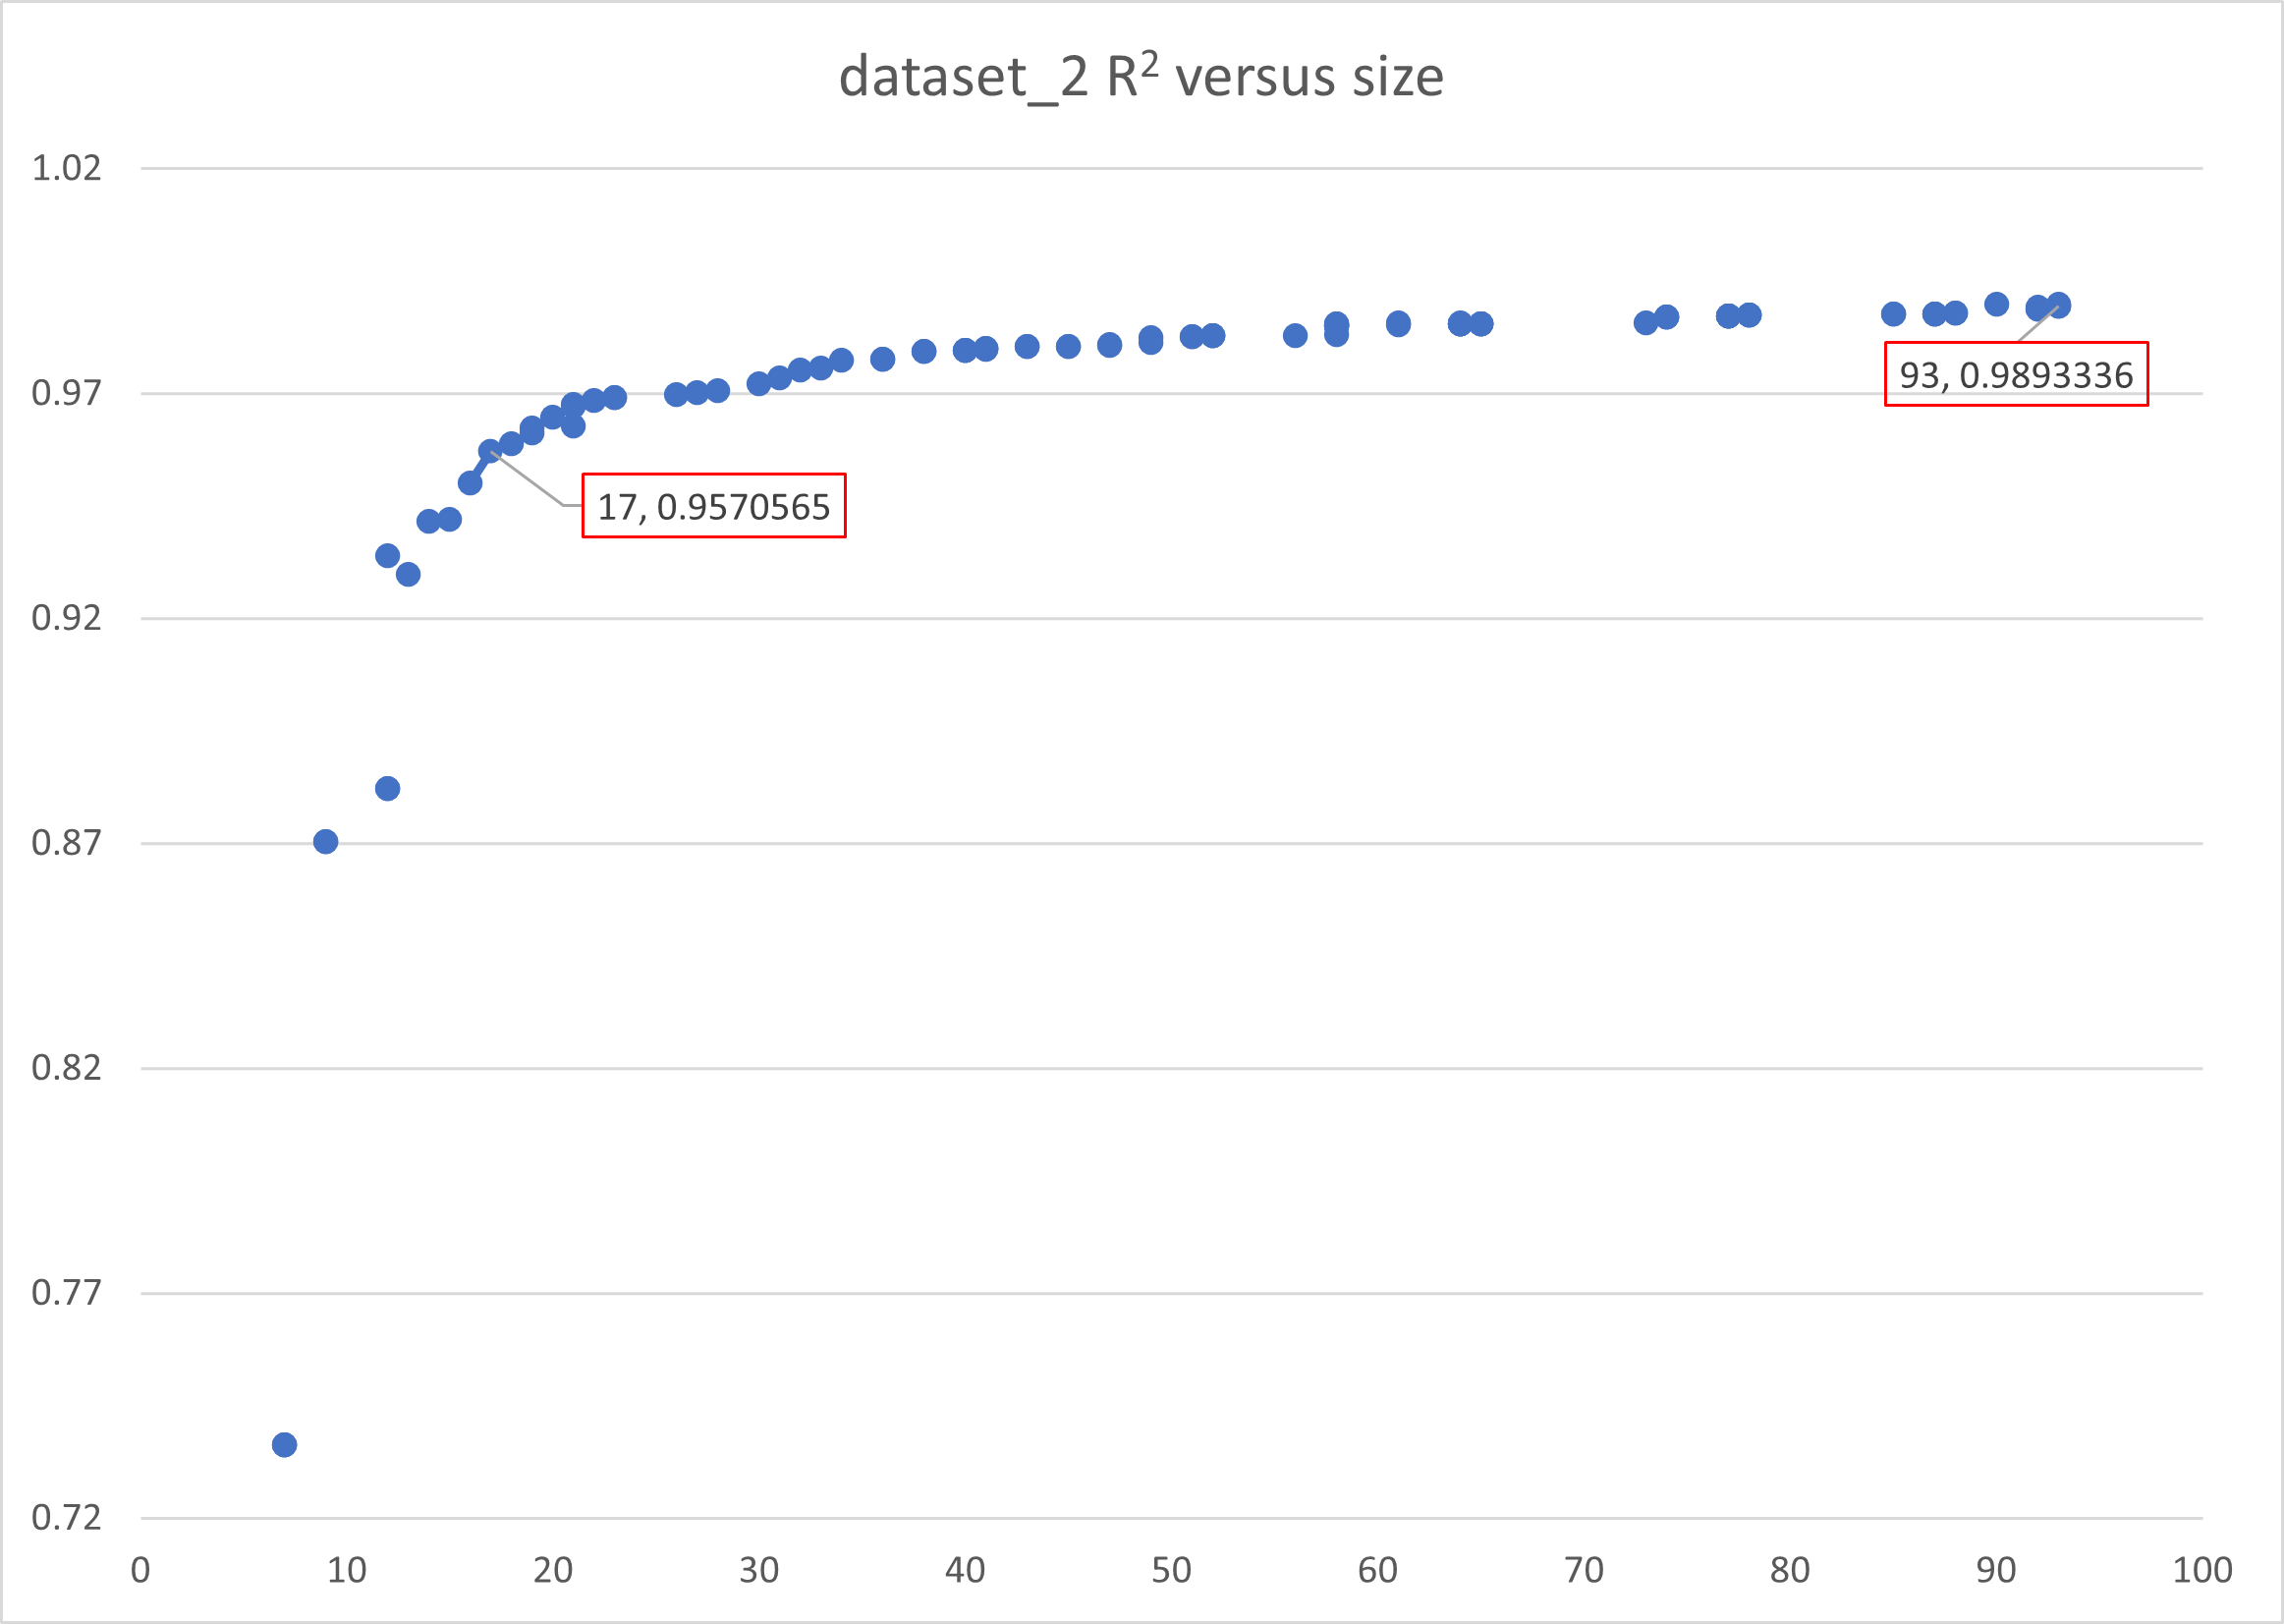
\includegraphics[width=0.95\linewidth]{solutions2.png}
  \label{fig:sfig2}
  
\end{subfigure}
\begin{subfigure}{1\textwidth}
  \centering
  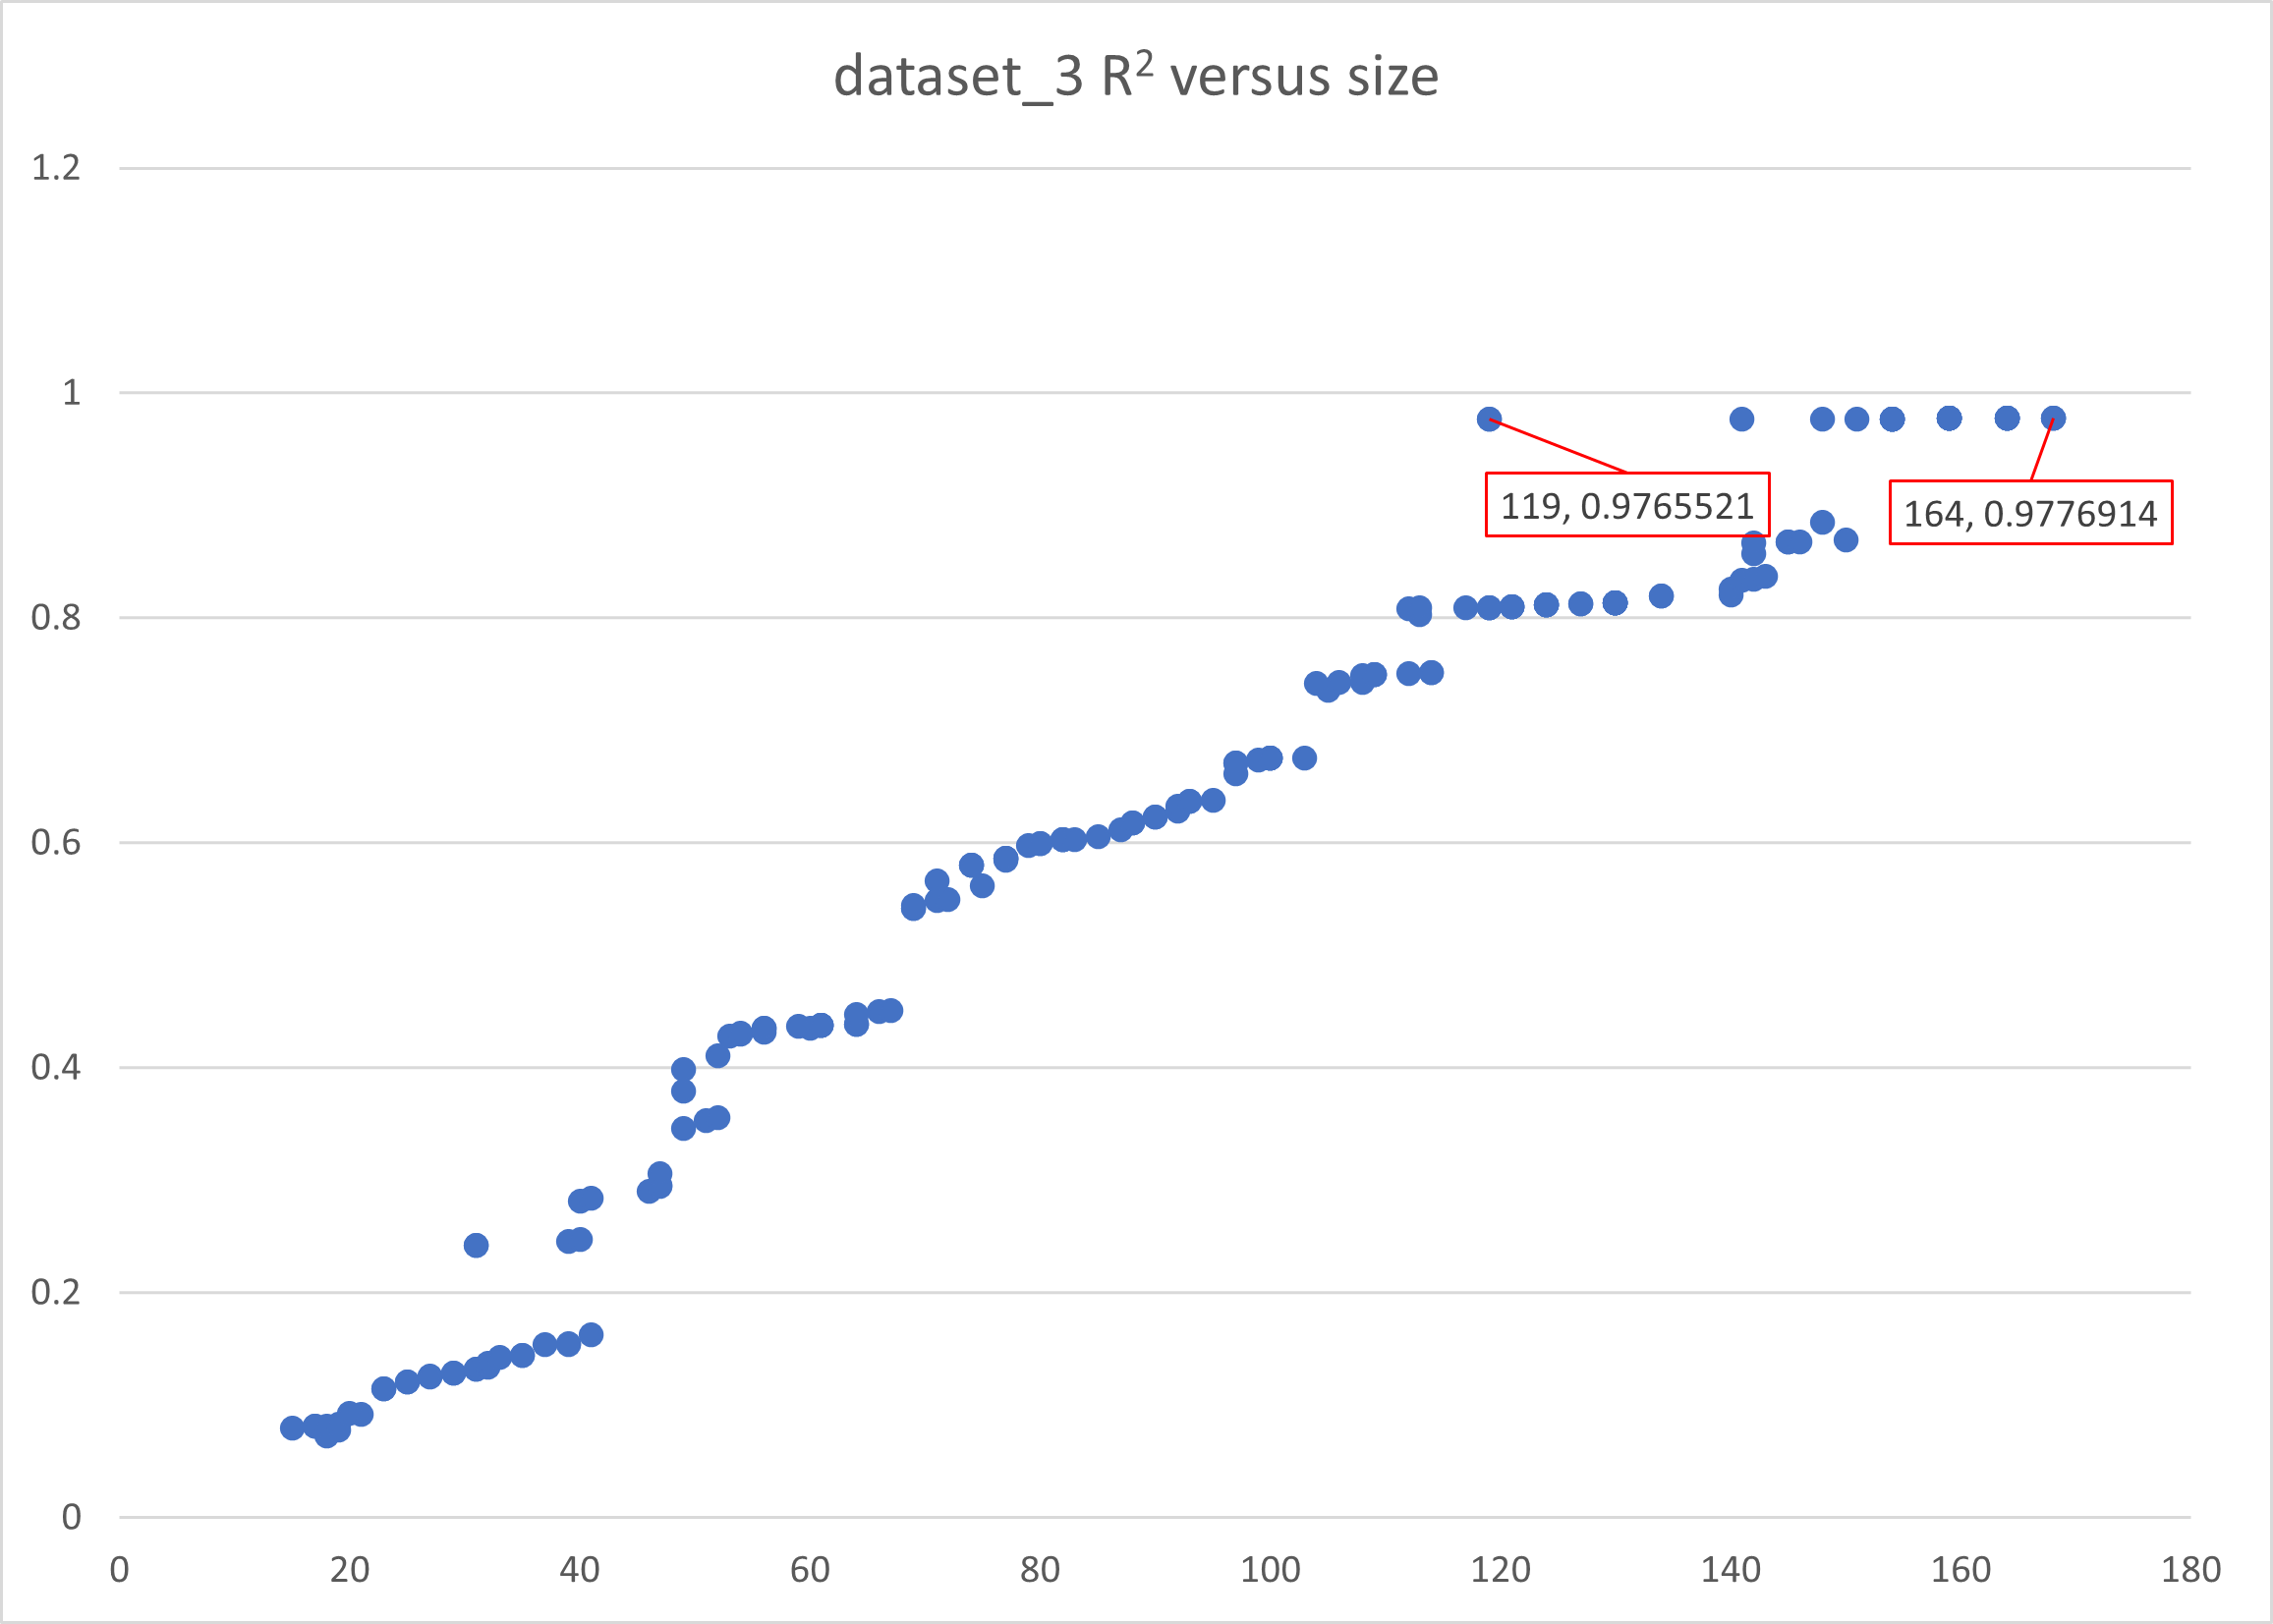
\includegraphics[width=0.5\linewidth]{solutions3.png}
  \label{fig:sfig3}
\end{subfigure}
\caption{Best trade-off solutions w.r.t. size and $R^2$ (step 2).}
\label{fig:fig_tradeoff}
\end{figure}

\bibliographystyle{vancouver}
\bibliography{bib}
 
\end{document}
